\documentclass[mathserif,serif]{beamer}
\usepackage{tabularx}
\setbeamertemplate{footline}[frame number]
% \useoutertheme{infolines}
\usepackage{slidesphysics}
\graphicspath{{../plot/}}

\title[]{Signal Optimization}
\author[]
{
Samuel Lo \inst{1}
\and
Yanjun Tu  \inst{1}
\and
Dongliang Zhang  \inst{2}
}
\institute[]
{
\inst{1}
The University of Hong Kong
\and
\inst{2}
University of Michigan
}
\date[]{\today}

\newcommand\Wider[2][3em]{%
\makebox[\linewidth][c]{%
\begin{minipage}{\dimexpr\textwidth+#1\relax}
\raggedright
\centering#2
\end{minipage}%
}%
}

\begin{document}
\frame{\titlepage}

\begin{frame}{Introduction}
\begin{itemize}
\item In this week, I am so confused that what I should do.
\begin{itemize}
\item Wednesday: Jeanette send me the to-do-list: Dani and I should agree on SR optimization (compare and agree on the final signal selection cuts), and Dongliang think it is good.
\item Thursday to Fridays: try to talk with Dani, and follow Dani's suggestion, just cross-check the yields from Dani's cut, and wait for her result.
\item Weekend: Dongliang think that I need to develop my tool to do my own optimization, cannot wait for Dani's result. I follow Dongliang's suggestion, and start to develop my code.
\item Monday: Dani has new results, but I need to find my optimized cut first, and want to compare my optimized cut with her.
\item Tuesday: Get some result for my own optimization, Jeanette knows I am doing my own optimization. Jeanette think I should not do my own optimization, but Dongliang do not think so.
\end{itemize}
\item Used the updated cross section for signal.
\item See separate slides for N-1 plots
\end{itemize}
\end{frame}

\section{optimization}
\begin{frame}{Method to deal with low statistics}
\begin{itemize}
\item If the weighted yield for a type of BG is negative, set the weighted yield to 0.
\item Weighted yield for signal need to be larger than 1.
\item nSig/nSigError $>$ 2.
\item If unweighted yield for total BG is 0, set the weighted yield to 1.
\item For METRel, pt1 and pt2, there is no upper cut if gain in significance $<$ 20\%.
\item For mlj/mljj, there is no lower cut.
\end{itemize}
\end{frame}

\begin{frame}{significance table}
\begin{itemize}
\item The optimized cuts for (175,0) signal point can be used.
\item Combined significance: \\
(175,0): 11.9, (165,35): 4.2, (400,0): 2.9
\end{itemize}
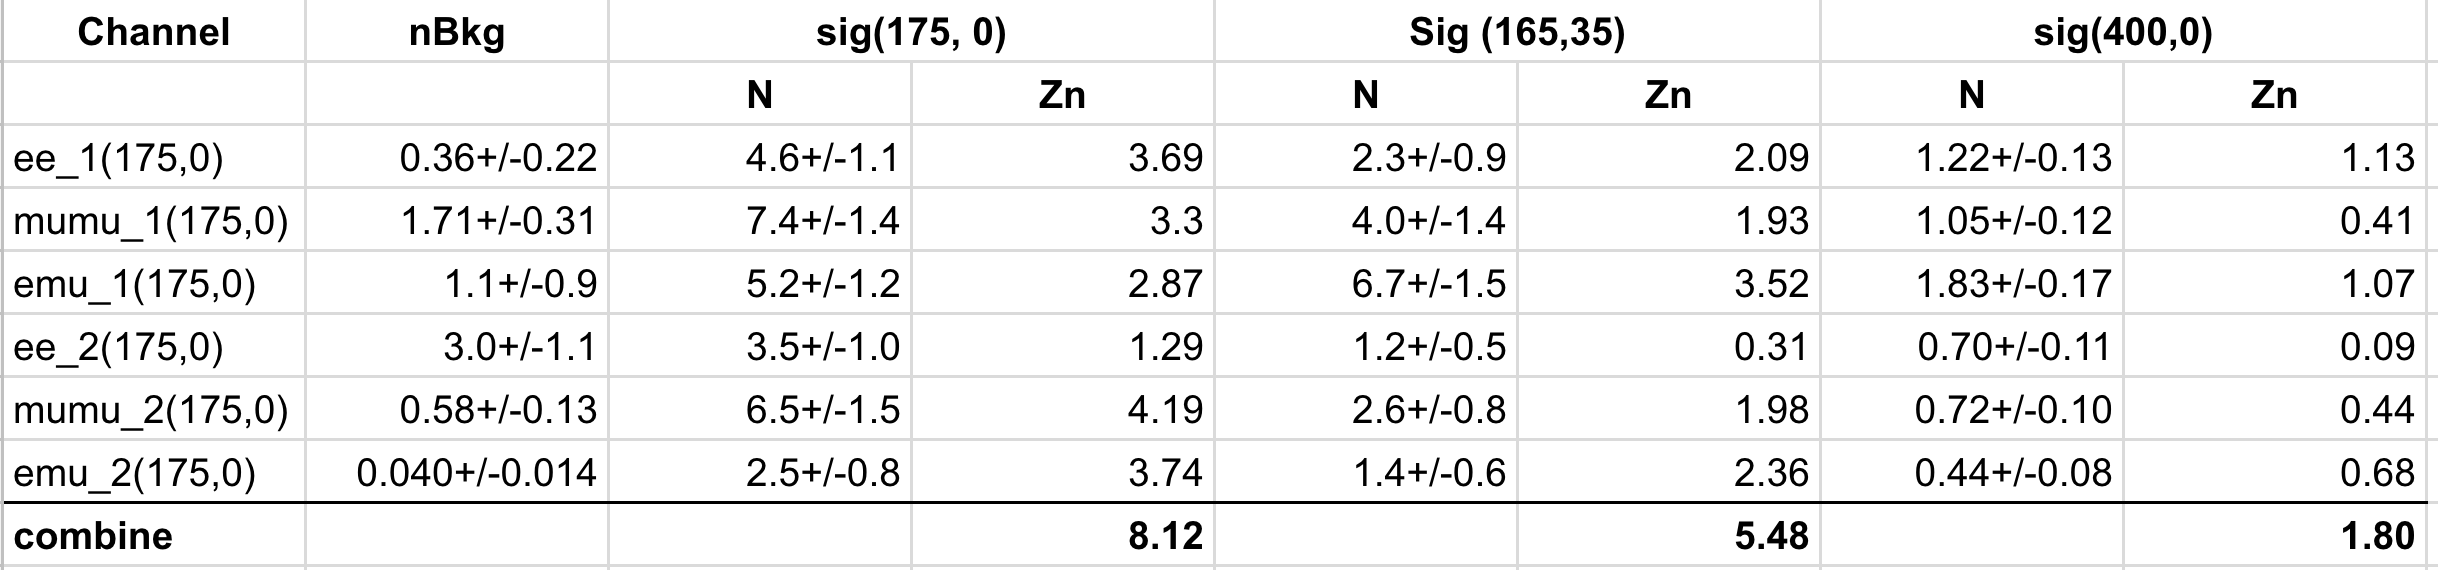
\includegraphics[width=\textwidth]{data/optimization/dongliang.png}
\end{frame}

\subsection{Yields table}
\begin{frame}{optimization}
\tiny
SR\_SS\_ee\_1\_opt: (162.5,12.5): \\
$\pt^{l1}$ $\geq 65$ \\
$\pt^{l2}$ $\geq 25$ \\
$|\Delta\eta_{ll}|$ $<1.5$ \\
$m_{\text{eff}}$ $\geq 200$ \\
$m_{\text{T}}^{\text{max}}$ $\geq 125$ \\
$m_{lj}$/$m_{ljj}$ $<105$ \\

\begin{tabular}{|c|c|c|}
\hline
& Number of events & Significance \\
\hline
VV & $4.515926\pm1.236724$ (943) & \\
\hline
V$+\gamma$ & $2.826692\pm1.288853$ (22) & \\
\hline
W+jets & $1.861954\pm1.779229$ (24) & \\
\hline
$t\bar{t}$ & $1.043981\pm0.864537$ (2) & \\
\hline
VVV & $0.245094\pm0.054352$ (29) & \\
\hline
single top & $0.204645\pm0.204645$ (1) & \\
\hline
$t\bar{t}+V$ & $0.090799\pm0.024928$ (23) & \\
\hline
Higgs & $0.006649\pm0.007073$ (3) & \\
\hline
Z+jets & $0.004363\pm0.004363$ (1) & \\
\hline
multi top & $0.000000\pm0.000000$ (0) & \\
\hline
Total BG & $10.800103\pm2.673805$ (1048) & \\
\hline
(162.5,12.5) & $3.06\pm0.64$ (28) &$0.34$\\
\hline
(175.0,0.0) & $2.07\pm0.61$ (15) &$0.16$\\
\hline
(450.0,0.0) & $0.13\pm0.06$ (4) &$-0.22$\\
\hline

\end{tabular}
\end{frame}

\begin{frame}{optimization}
\tiny
SR\_SS\_mumu\_1\_opt: (162.5,12.5): \\
$\pt^{l1}$ $\geq 55$ \\
$\pt^{l2}$ $\geq 20$ \\
$|\Delta\eta_{ll}|$ $<3$ \\
$m_{\text{eff}}$ $\geq 180$ \\
$m_{\text{T}}^{\text{max}}$ $\geq 105$ \\
$m_{lj}$/$m_{ljj}$ $<120$ \\
$\pt^{ll}$ $\geq 20$ \\

\begin{tabular}{|c|c|c|}
\hline
& Number of events & Significance \\
\hline
VV & $17.020370\pm1.037403$ (2574) & \\
\hline
Higgs & $2.049885\pm0.927366$ (8) & \\
\hline
W+jets & $1.411420\pm0.760263$ (7) & \\
\hline
VVV & $0.511978\pm0.073628$ (78) & \\
\hline
$t\bar{t}$ & $0.380504\pm0.380504$ (1) & \\
\hline
single top & $0.235893\pm0.235893$ (1) & \\
\hline
$t\bar{t}+V$ & $0.146444\pm0.030466$ (42) & \\
\hline
Z+jets & $0.019222\pm0.019222$ (1) & \\
\hline
V$+\gamma$ & $0.000000\pm0.000000$ (0) & \\
\hline
multi top & $0.000000\pm0.000000$ (0) & \\
\hline
Total BG & $21.775715\pm1.649654$ (2712) & \\
\hline
(162.5,12.5) & $10.66\pm1.39$ (83) &$1.13$\\
\hline
(202.5,72.5) & $3.81\pm0.90$ (29) &$0.32$\\
\hline
(450.0,0.0) & $0.17\pm0.08$ (5) &$-0.16$\\
\hline

\end{tabular}
\end{frame}

\begin{frame}{optimization}
\tiny
SR\_SS\_emu\_1\_opt: (162.5,12.5): \\
$\pt^{l1}$ $\geq 25$ \\
$\pt^{l2}$ $\geq 20$ \\
$|\Delta\eta_{ll}|$ $<4$ \\
$m_{\text{eff}}$ $\geq 190$ \\
$m_{\text{T}}^{\text{max}}$ $\geq 120$ \\
$m_{lj}$/$m_{ljj}$ $<95$ \\
$\pt^{ll}$ $\geq 30$ \\

\begin{tabular}{|c|c|c|}
\hline
& Number of events & Significance \\
\hline
VV & $6.213731\pm0.577077$ (956) & \\
\hline
Higgs & $1.003877\pm0.754074$ (8) & \\
\hline
W+jets & $0.695577\pm0.502594$ (5) & \\
\hline
V$+\gamma$ & $0.563608\pm0.254711$ (8) & \\
\hline
$t\bar{t}$ & $0.427347\pm0.427347$ (1) & \\
\hline
VVV & $0.329297\pm0.059250$ (44) & \\
\hline
single top & $0.129181\pm0.129181$ (1) & \\
\hline
$t\bar{t}+V$ & $0.029876\pm0.018387$ (20) & \\
\hline
multi top & $0.000000\pm0.000000$ (0) & \\
\hline
Z+jets & $0.000000\pm0.000000$ (0) & \\
\hline
Total BG & $9.392493\pm1.192597$ (1043) & \\
\hline
(162.5,12.5) & $6.22\pm0.90$ (58) &$1.17$\\
\hline
(175.0,0.0) & $5.91\pm1.03$ (42) &$1.11$\\
\hline
(450.0,0.0) & $0.45\pm0.14$ (12) &$-0.09$\\
\hline

\end{tabular}
\end{frame}

\begin{frame}{optimization}
\tiny
SR\_SS\_ee\_2\_opt: (175, 0): \\
$\pt$ of the leading lepton $\geq 35$ \\
$\pt$ of the subleading lepton $\geq 20$ \\
Dilepton $\pt$ $\geq 40$ \\
$m_{T2}$ $\geq 60$ \\
$E_{\text{T}}^{\text{miss,rel}}$ $\geq 20$ \\
$m_{\text{eff}}$ $\geq 100$ \\
$m_{\text{T}}^{\text{max}}$ $\geq 110$ \\
$m_{lj}$/$m_{ljj}$ $<120$ \\

\begin{tabular}{|c|c|c|}
\hline
& Number of events & Significance \\
\hline
VV & $4.831508\pm0.477421$ (1038) & \\
\hline
$t\bar{t}$ & $1.275492\pm0.650886$ (4) & \\
\hline
V$+\gamma$ & $1.020866\pm0.491290$ (7) & \\
\hline
Higgs & $0.532657\pm0.523089$ (13) & \\
\hline
$t\bar{t}+V$ & $0.213028\pm0.034466$ (87) & \\
\hline
VVV & $0.179405\pm0.047530$ (26) & \\
\hline
single top & $0.161341\pm0.161341$ (1) & \\
\hline
multi top & $0.000000\pm0.000000$ (0) & \\
\hline
Z+jets & $0.000000\pm0.000000$ (0) & \\
\hline
W+jets & $-0.079334\pm0.357300$ (3) & \\
\hline
Total BG & $8.214297\pm1.150527$ (1179) & \\
\hline
(162.5,12.5) & $5.54\pm0.96$ (47) &$1.12$\\
\hline
(175.0,0.0) & $3.25\pm0.92$ (21) &$0.61$\\
\hline
(450.0,0.0) & $0.28\pm0.13$ (6) &$-0.13$\\
\hline

\end{tabular}
\end{frame}

\begin{frame}{optimization}
\tiny
SR\_SS\_mumu\_2\_opt: (162.5,12.5): \\
$\pt^{l1}$ $\geq 25$ \\
$\pt^{l2}$ $\geq 30$ \\
$\pt^{ll}$ $\geq 30$ \\
$m_{T2}$ $\geq 20$ \\
$|\Delta\eta_{ll}|$ $<1.5$ \\
$E_{\text{T}}^{\text{miss,rel}}$ $\geq 35$ \\
$m_{\text{eff}}$ $\geq 220$ \\
$m_{\text{T}}^{\text{max}}$ $\geq 80$ \\
$m_{lj}$/$m_{ljj}$ $<120$ \\

\begin{tabular}{|c|c|c|}
\hline
& Number of events & Significance \\
\hline
Z+jets & $0.000000\pm0.000000$ (0) & \\
\hline
W+jets & $0.000000\pm0.000000$ (0) & \\
\hline
$t\bar{t}$ & $0.000000\pm0.000000$ (0) & \\
\hline
single top & $0.000000\pm0.000000$ (0) & \\
\hline
$t\bar{t}+V$ & $0.047645\pm0.019584$ (29) & \\
\hline
multi top & $0.000000\pm0.000000$ (0) & \\
\hline
VV & $2.423662\pm0.268231$ (636) & \\
\hline
V$+\gamma$ & $0.000000\pm0.000000$ (0) & \\
\hline
VVV & $0.099616\pm0.056583$ (6) & \\
\hline
Higgs & $0.392183\pm0.393018$ (5) & \\
\hline
Total BG & $2.963105\pm0.479579$ (676) & \\
\hline
(162.5,12.5) & $4.93\pm0.71$ (52) &$1.82$\\
\hline
(202.5,72.5) & $1.32\pm0.39$ (12) &$0.39$\\
\hline
(450.0,0.0) & $0.36\pm0.11$ (11) &$-0.07$\\
\hline

\end{tabular}
\end{frame}

\begin{frame}{optimization}
\tiny
SR\_SS\_emu\_2\_opt: (162.5,12.5): \\
$\pt^{l1}$ $\geq 25$ \\
$\pt^{l2}$ $\geq 20$ \\
$|\Delta\eta_{ll}|$ $<2.5$ \\
$E_{\text{T}}^{\text{miss,rel}}$ $\geq 80$ \\
$m_{\text{eff}}$ $\geq 260$ \\
$m_{\text{T}}^{\text{max}}$ $\geq 80$ \\
$m_{lj}$/$m_{ljj}$ $<115$ \\

\begin{tabular}{|c|c|c|}
\hline
& Number of events & Significance \\
\hline
Z+jets & $0.000000\pm0.000000$ (0) & \\
\hline
W+jets & $0.065759\pm0.065759$ (1) & \\
\hline
$t\bar{t}$ & $0.000000\pm0.000000$ (0) & \\
\hline
single top & $0.000000\pm0.000000$ (0) & \\
\hline
$t\bar{t}+V$ & $0.022601\pm0.009890$ (14) & \\
\hline
multi top & $0.000000\pm0.000000$ (0) & \\
\hline
VV & $0.807029\pm0.141785$ (185) & \\
\hline
V$+\gamma$ & $0.000000\pm0.000000$ (0) & \\
\hline
VVV & $0.018543\pm0.015652$ (4) & \\
\hline
Higgs & $0.003496\pm0.003286$ (6) & \\
\hline
Total BG & $0.917429\pm0.157419$ (210) & \\
\hline
Signal (175, 0) & $6.79\pm1.34$ (29) &$3.80$\\
\hline
Signal (165, 35) & $5.36\pm1.15$ (22) &$3.16$\\
\hline
Signal (400, 0) & $1.17\pm0.13$ (99) &$0.70$\\
\hline

\end{tabular}
\end{frame}



\section{Conclusion}
\begin{frame}{Conclusion}
\begin{itemize}
\item Conclusion:
\begin{itemize}
\item We should see significant excess if the signal exist
\item We can exclude the signal if they are not exist
\end{itemize}
\item Few issues need to further study:
\begin{itemize}
\item The global maximum for significance is difficult to find.
\item The low statistics of background sample.
\item need to understand some of the optimization results.
\end{itemize}
\end{itemize}
\end{frame}

\section{Plan}
\begin{frame}{Plan}
\begin{itemize}
\item Dani and Samuel will agree on the SR selection (compare and agree on the final signal selection cuts).
\item Dongliang and Samuel will work on data/MC plots after pre-selection level (all lepton cuts, possibly also jets and b-jets cuts).
\item Plot the electron eta to make a decision about whether we use the electrons in the crack region.
\item Estimate charge flip BG and fake BG from data, both in SR and pre-selection level.
\end{itemize}
\end{frame}

\begin{frame}
\begin{center}
\huge
Backup
\end{center}
\end{frame}

\begin{frame}{Selection in run1 SR}
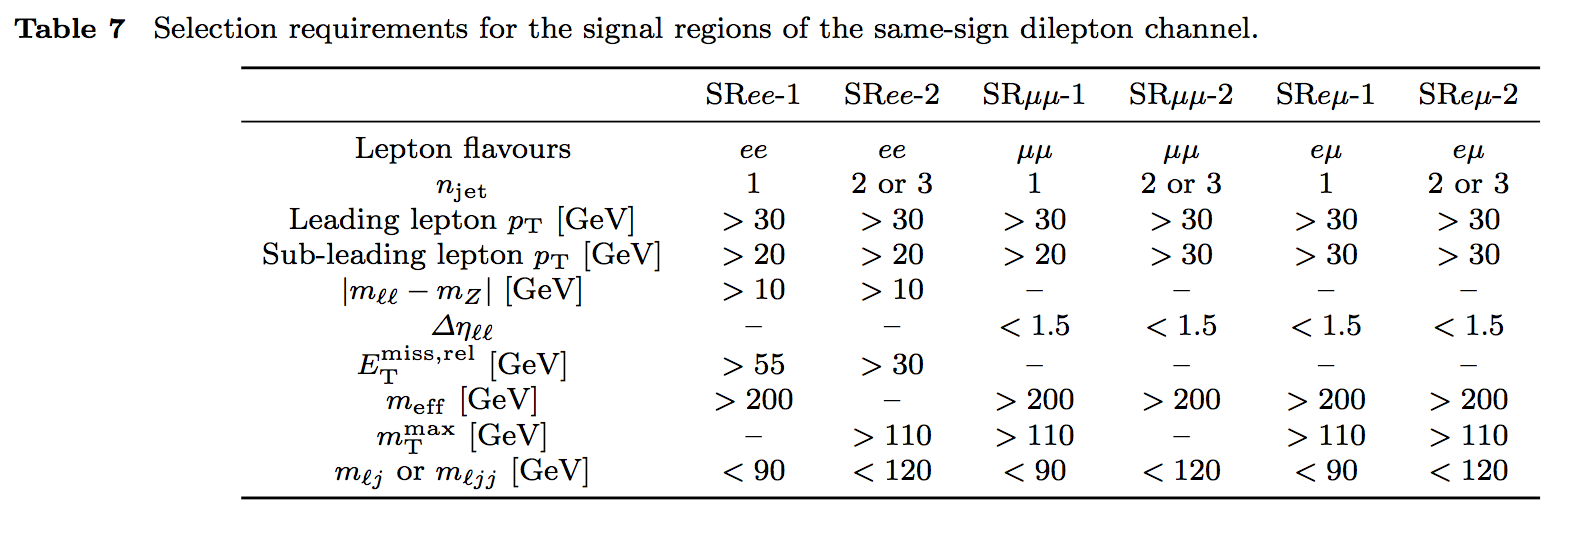
\includegraphics[width=\textwidth]{data/photo/SRcutrun1.png} \\
\url{https://arxiv.org/pdf/1501.07110.pdf}
\end{frame}

\begin{frame}
\frametitle{significance calculation}
\begin{itemize}
\item RooStats::NumberCountingUtils::BinomialExpZ(S,B,$\delta$B)
\item $\delta$B = 0.3
\end{itemize}
\end{frame}

\begin{frame}[fragile]
\frametitle{Signal sample}
\small
Sample Name(p2972 tag):
\tiny
\begin{verbatim}
mc15_13TeV.993820.MGPy8EG_A14N13LO_C1N2_Wh_2L_175_0.merge.DAOD_SUSY2.e5678_a766_a821_r7676_p2949_p2972
mc15_13TeV.993821.MGPy8EG_A14N13LO_C1N2_Wh_2L_165_35.merge.DAOD_SUSY2.e5678_a766_a821_r7676_p2949_p2972
mc15_13TeV.993822.MGPy8EG_A14N13LO_C1N2_Wh_2L_400_0.merge.DAOD_SUSY2.e5678_a766_a821_r7676_p2949_p2972
\end{verbatim}
\end{frame}

\begin{frame}[fragile]
\frametitle{Data}
\small
use both 2015 and 2016 data (3212.96 + 32861.6) /pb
\tiny
\begin{verbatim}
GRL:
GoodRunsLists/data16_13TeV/20161101/physics_25ns_20.7.xml
GoodRunsLists/data15_13TeV/20160720/physics_25ns_20.7.xml
\end{verbatim}
\end{frame}

\begin{frame}{MC BG}
p-tag: p2949
\end{frame}

\begin{frame}[fragile]
\small
Trigger list:\\
\scriptsize
\begin{verbatim}
2015
HLT_2e12_lhloose_L12EM10VH
HLT_e17_lhloose_mu14
HLT_mu18_mu8noL1

2016(A-D3)
HLT_2e17_lhvloose_nod0
HLT_e17_lhloose_nod0_mu14
HLT_mu20_mu8noL1

2016(D3-)
HLT_2e17_lhvloose_nod0
HLT_e17_lhloose_nod0_mu14
HLT_mu22_mu8noL1
\end{verbatim}
\end{frame}

\begin{frame}{Object Definitions}
\small
Tool: AnalysisBase 2.4.31, SUSYTools-00-08-60\\

\centering
\begin{table}
\small
\begin{tabularx}{\textwidth}{p{1.5cm} | p{3cm} | p{3cm} | p{3cm}}
& \textbf{Electron} & \textbf{Muon} & \textbf{Jet}\\
\hline
\textbf{Baseline}
& - $p_T>10$ GeV \newline - $|\eta^{cluster}| < 2.47$ \newline - LooseAndBLayerLLH
& - $p_T>10$ GeV \newline - $|\eta| < 2.7$ \newline - Medium
& - $p_T>20$ GeV \\
\hline
\textbf{Signal}
& - $p_T > 25$ GeV \newline - $|\eta^{cluster}| < 2.47$ \newline - TightLLH \newline - GradientLoose \newline - $|z_0 \sin \theta| < 0.5$mm \newline - $|d_0/\sigma_{d_0}| < 5$
& - $p_T > 25$ GeV \newline - $|\eta| < 2.7$ \newline - Medium \newline - GradientLoose \newline - $|z_0 \sin \theta| < 0.5$mm \newline - $|d_0/\sigma_{d_0}| < 3$
& - $p_T > 20$ GeV \newline - $|\eta|<2.8$ \newline \newline - $|JVT| > 0.59$ \newline if $p_T < 60$ GeV \newline and $|\eta| < 2.4$
\end{tabularx}
\end{table}

\raggedright
Selection:
\begin{itemize}
%\item Trigger selection
\item Exactly 2 baseline leptons and exactly 2 signal leptons
\end{itemize}

\tiny
Note: \\
Pileup reweighting is applied. \\
Scale factor for reconstruction, isolation, ID and trigger is applied.
\end{frame}

\begin{frame}
\frametitle{Definition of jets}
\normalsize
\begin{itemize}
\item Central jets: $\pt>20$ GeV, $|\eta|<2.4$, no b-tagged
\item B-jets: b-tagged
\end{itemize}
\end{frame}

\begin{frame}
\frametitle{definition of variables}
\normalsize
\begin{itemize}
\item HT: Sum of the $p_T$ of all signal jets and the two leptons.
\item R2 = MET / (MET + pt1 + pt2)
\item l12\_dPhi: difference in phi between the two leptons.
\item l12\_MET\_dPhi: difference in phi between MET and the sum of 4-momentum of the two leptons.
\end{itemize}
\end{frame}

\subsection{``N-1'' plots}
\begin{frame}{$p_T^{l1}$}
\Wider{
\includegraphics[width=0.49\textwidth]{pt1_SR_SS_jet1_opt_0}
\includegraphics[width=0.49\textwidth]{pt1_SR_SS_jet23_opt_0}
}
\end{frame}

\begin{frame}{$p_T^{l2}$}
\Wider{
\includegraphics[width=0.49\textwidth]{pt2_SR_SS_jet1_opt_0}
\includegraphics[width=0.49\textwidth]{pt2_SR_SS_jet23_opt_0}
}
\end{frame}

\begin{frame}{$|\Delta\eta_{ll}|$}
\Wider{
\includegraphics[width=0.49\textwidth]{dEta_SR_SS_jet1_opt_0}
\includegraphics[width=0.49\textwidth]{dEta_SR_SS_jet23_opt_0}
}
\end{frame}

\begin{frame}{$E_{\text{T}}^{\text{miss}}$}
\Wider{
\includegraphics[width=0.49\textwidth]{MET_SR_SS_jet1_opt_0}
\includegraphics[width=0.49\textwidth]{MET_SR_SS_jet23_opt_0}
}
\end{frame}

\begin{frame}{$m_{\text{eff}}$}
\Wider{
\includegraphics[width=0.49\textwidth]{meff_SR_SS_jet1_opt_0}
\includegraphics[width=0.49\textwidth]{meff_SR_SS_jet23_opt_0}
}
\end{frame}

\begin{frame}{$m_{\text{T}}^{l1}$}
\Wider{
\includegraphics[width=0.49\textwidth]{mt1_SR_SS_jet1_opt_0}
\includegraphics[width=0.49\textwidth]{mt1_SR_SS_jet23_opt_0}
}
\end{frame}

\begin{frame}{$m_{lj}$/$m_{ljj}$}
\Wider{
\includegraphics[width=0.49\textwidth]{mlj_SR_SS_jet1_opt_0}
\includegraphics[width=0.49\textwidth]{mlj_SR_SS_jet23_opt_0}
}
\end{frame}

\begin{frame}{$m_{T2}$}
\Wider{
\includegraphics[width=0.49\textwidth]{mTtwo_SR_SS_jet1_opt_0}
\includegraphics[width=0.49\textwidth]{mTtwo_SR_SS_jet23_opt_0}
}
\end{frame}


%\begin{frame}{Expected number of events \\ For SR\_SS\_ee\_1}
\vspace{5mm}
\begin{tabular}{|c|c|c|}
\hline
& Number of events & Significance \\
\hline
Z+jets & $18.9\pm19.8$ & \\
\hline
W+jets & $3.3\pm2.1$ & \\
\hline
top & $69.1\pm5.8$ & \\
\hline
VV & $14.1\pm2.0$ & \\
\hline
V$+\gamma$ & $12.2\pm5.5$ & \\
\hline
VVV & $0.4\pm0.1$ & \\
\hline
Total BG & $117.9\pm21.6$ & \\
\hline
Signal (175, 0) & $7.1\pm1.2$ &$-0.009$\\
\hline
Signal (165, 35) & $2.4\pm0.4$ &$-0.134$\\
\hline
Signal (400, 0) & $9.8\pm0.8$ &$0.062$\\
\hline

\end{tabular}
\end{frame}

\begin{frame}{Expected number of events \\ For SR\_SS\_mumu\_1}
\vspace{5mm}
\begin{tabular}{|c|c|c|}
\hline
& Number of events & Significance \\
\hline
Z+jets & $6.4\pm6.5$ & \\
\hline
W+jets & $0.4\pm0.4$ & \\
\hline
top & $4.0\pm0.8$ & \\
\hline
VV & $7.1\pm0.7$ & \\
\hline
V$+\gamma$ & $0.0\pm0.0$ & \\
\hline
VVV & $0.3\pm0.1$ & \\
\hline
Total BG & $18.3\pm6.6$ & \\
\hline
Signal (175, 0) & $5.4\pm0.8$ &$0.531$\\
\hline
Signal (165, 35) & $2.6\pm0.5$ &$0.159$\\
\hline
Signal (400, 0) & $9.0\pm0.9$ &$0.960$\\
\hline

\end{tabular}
\end{frame}

\begin{frame}{Expected number of events \\ For SR\_SS\_emu\_1}
\vspace{5mm}
\begin{tabular}{|c|c|c|}
\hline
& Number of events & Significance \\
\hline
Z+jets & $0.1\pm0.0$ & \\
\hline
W+jets & $5.0\pm2.4$ & \\
\hline
top & $39.9\pm3.6$ & \\
\hline
VV & $14.9\pm1.8$ & \\
\hline
V$+\gamma$ & $1.5\pm0.5$ & \\
\hline
VVV & $0.4\pm0.1$ & \\
\hline
Total BG & $61.9\pm4.7$ & \\
\hline
Signal (175, 0) & $8.1\pm1.2$ &$0.191$\\
\hline
Signal (165, 35) & $5.5\pm0.6$ &$0.068$\\
\hline
Signal (400, 0) & $15.0\pm1.1$ &$0.501$\\
\hline

\end{tabular}
\end{frame}

\begin{frame}{Expected number of events \\ For SR\_SS\_ee\_2}
\vspace{5mm}
\begin{tabular}{|c|c|c|}
\hline
& Number of events & Significance \\
\hline
VV & $2.8\pm0.4$ & \\
\hline
V$+\gamma$ & $2.3\pm1.2$ & \\
\hline
Total BG & $5.1\pm1.2$ & \\
\hline
Signal (400, 380) & $0.0\pm0.0$ &$-0.229$\\
\hline
Signal (500, 450) & $0.1\pm0.0$ &$-0.188$\\
\hline
Signal (400, 300) & $0.8\pm0.1$ &$0.045$\\
\hline
Signal (400, 200) & $0.5\pm0.1$ &$-0.040$\\
\hline
Signal (400, 100) & $0.4\pm0.2$ &$-0.088$\\
\hline

\end{tabular}
\end{frame}

\begin{frame}{Expected number of events \\ For SR\_SS\_mumu\_2}
\vspace{5mm}
\begin{tabular}{|c|c|c|}
\hline
& Number of events & Significance \\
\hline
Z+jets & $89.3\pm27.3$ & \\
\hline
W+jets & $1.1\pm0.6$ & \\
\hline
top & $10.7\pm1.5$ & \\
\hline
VV & $16.3\pm0.7$ & \\
\hline
V$+\gamma$ & $2.5\pm1.3$ & \\
\hline
VVV & $0.3\pm0.1$ & \\
\hline
Total BG & $120.1\pm27.4$ & \\
\hline
Signal (175, 0) & $9.7\pm1.3$ &$0.055$\\
\hline
Signal (165, 35) & $4.1\pm0.5$ &$-0.091$\\
\hline
Signal (400, 0) & $7.5\pm0.7$ &$-0.003$\\
\hline

\end{tabular}
\end{frame}

\begin{frame}{Expected number of events \\ For SR\_SS\_emu\_2}
\vspace{5mm}
\begin{tabular}{|c|c|c|}
\hline
& Number of events & Significance \\
\hline
VV & $6.0\pm0.4$ & \\
\hline
V$+\gamma$ & $1.1\pm0.8$ & \\
\hline
Total BG & $7.1\pm0.9$ & \\
\hline
Signal (400, 380) & $0.0\pm0.0$ &$-0.213$\\
\hline
Signal (500, 450) & $0.2\pm0.0$ &$-0.162$\\
\hline
Signal (400, 300) & $1.3\pm0.2$ &$0.163$\\
\hline
Signal (400, 200) & $0.8\pm0.1$ &$0.014$\\
\hline
Signal (400, 100) & $0.5\pm0.2$ &$-0.075$\\
\hline

\end{tabular}
\end{frame}


%\begin{frame}{For SR\_SS\_run1 \\ $\pt$ of the leading lepton}
\Wider[5em]{
\includegraphics[width=0.33\textwidth]{pt1_SR_SS_ee_1}
\includegraphics[width=0.33\textwidth]{pt1_SR_SS_mumu_1}
\includegraphics[width=0.33\textwidth]{pt1_SR_SS_emu_1} \\
\includegraphics[width=0.33\textwidth]{pt1_SR_SS_ee_2}
\includegraphics[width=0.33\textwidth]{pt1_SR_SS_mumu_2}
\includegraphics[width=0.33\textwidth]{pt1_SR_SS_emu_2}
}
\end{frame}

\begin{frame}{For SR\_SS\_run1 \\ $\pt$ of the subleading lepton}
\Wider[5em]{
\includegraphics[width=0.33\textwidth]{pt2_SR_SS_ee_1}
\includegraphics[width=0.33\textwidth]{pt2_SR_SS_mumu_1}
\includegraphics[width=0.33\textwidth]{pt2_SR_SS_emu_1} \\
\includegraphics[width=0.33\textwidth]{pt2_SR_SS_ee_2}
\includegraphics[width=0.33\textwidth]{pt2_SR_SS_mumu_2}
\includegraphics[width=0.33\textwidth]{pt2_SR_SS_emu_2}
}
\end{frame}

\begin{frame}{For SR\_SS\_run1 \\ $\eta$ of the leading lepton}
\Wider[5em]{
\includegraphics[width=0.33\textwidth]{eta1_SR_SS_ee_1}
\includegraphics[width=0.33\textwidth]{eta1_SR_SS_mumu_1}
\includegraphics[width=0.33\textwidth]{eta1_SR_SS_emu_1} \\
\includegraphics[width=0.33\textwidth]{eta1_SR_SS_ee_2}
\includegraphics[width=0.33\textwidth]{eta1_SR_SS_mumu_2}
\includegraphics[width=0.33\textwidth]{eta1_SR_SS_emu_2}
}
\end{frame}

\begin{frame}{For SR\_SS\_run1 \\ $\eta$ of the subleading lepton}
\Wider[5em]{
\includegraphics[width=0.33\textwidth]{eta2_SR_SS_ee_1}
\includegraphics[width=0.33\textwidth]{eta2_SR_SS_mumu_1}
\includegraphics[width=0.33\textwidth]{eta2_SR_SS_emu_1} \\
\includegraphics[width=0.33\textwidth]{eta2_SR_SS_ee_2}
\includegraphics[width=0.33\textwidth]{eta2_SR_SS_mumu_2}
\includegraphics[width=0.33\textwidth]{eta2_SR_SS_emu_2}
}
\end{frame}

\begin{frame}{For SR\_SS\_run1 \\ $\phi$ of the leading lepton}
\Wider[5em]{
\includegraphics[width=0.33\textwidth]{phi1_SR_SS_ee_1}
\includegraphics[width=0.33\textwidth]{phi1_SR_SS_mumu_1}
\includegraphics[width=0.33\textwidth]{phi1_SR_SS_emu_1} \\
\includegraphics[width=0.33\textwidth]{phi1_SR_SS_ee_2}
\includegraphics[width=0.33\textwidth]{phi1_SR_SS_mumu_2}
\includegraphics[width=0.33\textwidth]{phi1_SR_SS_emu_2}
}
\end{frame}

\begin{frame}{For SR\_SS\_run1 \\ $m_{ll}$}
\Wider[5em]{
\includegraphics[width=0.33\textwidth]{mll_SR_SS_ee_1}
\includegraphics[width=0.33\textwidth]{mll_SR_SS_mumu_1}
\includegraphics[width=0.33\textwidth]{mll_SR_SS_emu_1} \\
\includegraphics[width=0.33\textwidth]{mll_SR_SS_ee_2}
\includegraphics[width=0.33\textwidth]{mll_SR_SS_mumu_2}
\includegraphics[width=0.33\textwidth]{mll_SR_SS_emu_2}
}
\end{frame}

\begin{frame}{For SR\_SS\_run1 \\ Dilepton $\pt$}
\Wider[5em]{
\includegraphics[width=0.33\textwidth]{ptll_SR_SS_ee_1}
\includegraphics[width=0.33\textwidth]{ptll_SR_SS_mumu_1}
\includegraphics[width=0.33\textwidth]{ptll_SR_SS_emu_1} \\
\includegraphics[width=0.33\textwidth]{ptll_SR_SS_ee_2}
\includegraphics[width=0.33\textwidth]{ptll_SR_SS_mumu_2}
\includegraphics[width=0.33\textwidth]{ptll_SR_SS_emu_2}
}
\end{frame}

\begin{frame}{For SR\_SS\_run1 \\ $E_{\text{T}}^{\text{miss}}$}
\Wider[5em]{
\includegraphics[width=0.33\textwidth]{MET_SR_SS_ee_1}
\includegraphics[width=0.33\textwidth]{MET_SR_SS_mumu_1}
\includegraphics[width=0.33\textwidth]{MET_SR_SS_emu_1} \\
\includegraphics[width=0.33\textwidth]{MET_SR_SS_ee_2}
\includegraphics[width=0.33\textwidth]{MET_SR_SS_mumu_2}
\includegraphics[width=0.33\textwidth]{MET_SR_SS_emu_2}
}
\end{frame}

\begin{frame}{For SR\_SS\_run1 \\ $m_{T2}$}
\Wider[5em]{
\includegraphics[width=0.33\textwidth]{mTtwo_SR_SS_ee_1}
\includegraphics[width=0.33\textwidth]{mTtwo_SR_SS_mumu_1}
\includegraphics[width=0.33\textwidth]{mTtwo_SR_SS_emu_1} \\
\includegraphics[width=0.33\textwidth]{mTtwo_SR_SS_ee_2}
\includegraphics[width=0.33\textwidth]{mTtwo_SR_SS_mumu_2}
\includegraphics[width=0.33\textwidth]{mTtwo_SR_SS_emu_2}
}
\end{frame}

\begin{frame}{For SR\_SS\_run1 \\ $m_{\text{T}}$ of the leading lepton}
\Wider[5em]{
\includegraphics[width=0.33\textwidth]{mt1_SR_SS_ee_1}
\includegraphics[width=0.33\textwidth]{mt1_SR_SS_mumu_1}
\includegraphics[width=0.33\textwidth]{mt1_SR_SS_emu_1} \\
\includegraphics[width=0.33\textwidth]{mt1_SR_SS_ee_2}
\includegraphics[width=0.33\textwidth]{mt1_SR_SS_mumu_2}
\includegraphics[width=0.33\textwidth]{mt1_SR_SS_emu_2}
}
\end{frame}

\begin{frame}{For SR\_SS\_run1 \\ $m_{\text{T}}$ of the subleading lepton}
\Wider[5em]{
\includegraphics[width=0.33\textwidth]{mt2_SR_SS_ee_1}
\includegraphics[width=0.33\textwidth]{mt2_SR_SS_mumu_1}
\includegraphics[width=0.33\textwidth]{mt2_SR_SS_emu_1} \\
\includegraphics[width=0.33\textwidth]{mt2_SR_SS_ee_2}
\includegraphics[width=0.33\textwidth]{mt2_SR_SS_mumu_2}
\includegraphics[width=0.33\textwidth]{mt2_SR_SS_emu_2}
}
\end{frame}

\begin{frame}{For SR\_SS\_run1 \\ $\pt$ of the leading jet}
\Wider[5em]{
\includegraphics[width=0.33\textwidth]{jetpt_SR_SS_ee_1}
\includegraphics[width=0.33\textwidth]{jetpt_SR_SS_mumu_1}
\includegraphics[width=0.33\textwidth]{jetpt_SR_SS_emu_1} \\
\includegraphics[width=0.33\textwidth]{jetpt_SR_SS_ee_2}
\includegraphics[width=0.33\textwidth]{jetpt_SR_SS_mumu_2}
\includegraphics[width=0.33\textwidth]{jetpt_SR_SS_emu_2}
}
\end{frame}

\begin{frame}{For SR\_SS\_run1 \\ $\eta$ of the leading jet}
\Wider[5em]{
\includegraphics[width=0.33\textwidth]{jeteta_SR_SS_ee_1}
\includegraphics[width=0.33\textwidth]{jeteta_SR_SS_mumu_1}
\includegraphics[width=0.33\textwidth]{jeteta_SR_SS_emu_1} \\
\includegraphics[width=0.33\textwidth]{jeteta_SR_SS_ee_2}
\includegraphics[width=0.33\textwidth]{jeteta_SR_SS_mumu_2}
\includegraphics[width=0.33\textwidth]{jeteta_SR_SS_emu_2}
}
\end{frame}

\begin{frame}{For SR\_SS\_run1 \\ Number of jets}
\Wider[5em]{
\includegraphics[width=0.33\textwidth]{nJet_SR_SS_ee_1}
\includegraphics[width=0.33\textwidth]{nJet_SR_SS_mumu_1}
\includegraphics[width=0.33\textwidth]{nJet_SR_SS_emu_1} \\
\includegraphics[width=0.33\textwidth]{nJet_SR_SS_ee_2}
\includegraphics[width=0.33\textwidth]{nJet_SR_SS_mumu_2}
\includegraphics[width=0.33\textwidth]{nJet_SR_SS_emu_2}
}
\end{frame}

\begin{frame}{For SR\_SS\_run1 \\ Number of b-jets}
\Wider[5em]{
\includegraphics[width=0.33\textwidth]{nBJet_SR_SS_ee_1}
\includegraphics[width=0.33\textwidth]{nBJet_SR_SS_mumu_1}
\includegraphics[width=0.33\textwidth]{nBJet_SR_SS_emu_1} \\
\includegraphics[width=0.33\textwidth]{nBJet_SR_SS_ee_2}
\includegraphics[width=0.33\textwidth]{nBJet_SR_SS_mumu_2}
\includegraphics[width=0.33\textwidth]{nBJet_SR_SS_emu_2}
}
\end{frame}

\begin{frame}{For SR\_SS\_run1 \\ Number of central jets}
\Wider[5em]{
\includegraphics[width=0.33\textwidth]{nCJet_SR_SS_ee_1}
\includegraphics[width=0.33\textwidth]{nCJet_SR_SS_mumu_1}
\includegraphics[width=0.33\textwidth]{nCJet_SR_SS_emu_1} \\
\includegraphics[width=0.33\textwidth]{nCJet_SR_SS_ee_2}
\includegraphics[width=0.33\textwidth]{nCJet_SR_SS_mumu_2}
\includegraphics[width=0.33\textwidth]{nCJet_SR_SS_emu_2}
}
\end{frame}

\begin{frame}{For SR\_SS\_run1 \\ $\Delta\phi_{ll}$}
\Wider[5em]{
\includegraphics[width=0.33\textwidth]{l12_dPhi_SR_SS_ee_1}
\includegraphics[width=0.33\textwidth]{l12_dPhi_SR_SS_mumu_1}
\includegraphics[width=0.33\textwidth]{l12_dPhi_SR_SS_emu_1} \\
\includegraphics[width=0.33\textwidth]{l12_dPhi_SR_SS_ee_2}
\includegraphics[width=0.33\textwidth]{l12_dPhi_SR_SS_mumu_2}
\includegraphics[width=0.33\textwidth]{l12_dPhi_SR_SS_emu_2}
}
\end{frame}

\begin{frame}{For SR\_SS\_run1 \\ $\Delta\phi_{ll,\text{MET}}$}
\Wider[5em]{
\includegraphics[width=0.33\textwidth]{l12_MET_dPhi_SR_SS_ee_1}
\includegraphics[width=0.33\textwidth]{l12_MET_dPhi_SR_SS_mumu_1}
\includegraphics[width=0.33\textwidth]{l12_MET_dPhi_SR_SS_emu_1} \\
\includegraphics[width=0.33\textwidth]{l12_MET_dPhi_SR_SS_ee_2}
\includegraphics[width=0.33\textwidth]{l12_MET_dPhi_SR_SS_mumu_2}
\includegraphics[width=0.33\textwidth]{l12_MET_dPhi_SR_SS_emu_2}
}
\end{frame}

\begin{frame}{For SR\_SS\_run1 \\ $\Delta\phi_{\text{jet0,MET}}$}
\Wider[5em]{
\includegraphics[width=0.33\textwidth]{jets_MET_dPhi_SR_SS_ee_1}
\includegraphics[width=0.33\textwidth]{jets_MET_dPhi_SR_SS_mumu_1}
\includegraphics[width=0.33\textwidth]{jets_MET_dPhi_SR_SS_emu_1} \\
\includegraphics[width=0.33\textwidth]{jets_MET_dPhi_SR_SS_ee_2}
\includegraphics[width=0.33\textwidth]{jets_MET_dPhi_SR_SS_mumu_2}
\includegraphics[width=0.33\textwidth]{jets_MET_dPhi_SR_SS_emu_2}
}
\end{frame}

\begin{frame}{For SR\_SS\_run1 \\ $\Delta\eta_{ll}$}
\Wider[5em]{
\includegraphics[width=0.33\textwidth]{dEta_SR_SS_ee_1}
\includegraphics[width=0.33\textwidth]{dEta_SR_SS_mumu_1}
\includegraphics[width=0.33\textwidth]{dEta_SR_SS_emu_1} \\
\includegraphics[width=0.33\textwidth]{dEta_SR_SS_ee_2}
\includegraphics[width=0.33\textwidth]{dEta_SR_SS_mumu_2}
\includegraphics[width=0.33\textwidth]{dEta_SR_SS_emu_2}
}
\end{frame}

\begin{frame}{For SR\_SS\_run1 \\ $E_{\text{T}}^{\text{miss,rel}}$}
\Wider[5em]{
\includegraphics[width=0.33\textwidth]{METRel_SR_SS_ee_1}
\includegraphics[width=0.33\textwidth]{METRel_SR_SS_mumu_1}
\includegraphics[width=0.33\textwidth]{METRel_SR_SS_emu_1} \\
\includegraphics[width=0.33\textwidth]{METRel_SR_SS_ee_2}
\includegraphics[width=0.33\textwidth]{METRel_SR_SS_mumu_2}
\includegraphics[width=0.33\textwidth]{METRel_SR_SS_emu_2}
}
\end{frame}

\begin{frame}{For SR\_SS\_run1 \\ $m_{\text{eff}}$}
\Wider[5em]{
\includegraphics[width=0.33\textwidth]{meff_SR_SS_ee_1}
\includegraphics[width=0.33\textwidth]{meff_SR_SS_mumu_1}
\includegraphics[width=0.33\textwidth]{meff_SR_SS_emu_1} \\
\includegraphics[width=0.33\textwidth]{meff_SR_SS_ee_2}
\includegraphics[width=0.33\textwidth]{meff_SR_SS_mumu_2}
\includegraphics[width=0.33\textwidth]{meff_SR_SS_emu_2}
}
\end{frame}

\begin{frame}{For SR\_SS\_run1 \\ $m_{\text{T}}^{\text{max}}$}
\Wider[5em]{
\includegraphics[width=0.33\textwidth]{mtm_SR_SS_ee_1}
\includegraphics[width=0.33\textwidth]{mtm_SR_SS_mumu_1}
\includegraphics[width=0.33\textwidth]{mtm_SR_SS_emu_1} \\
\includegraphics[width=0.33\textwidth]{mtm_SR_SS_ee_2}
\includegraphics[width=0.33\textwidth]{mtm_SR_SS_mumu_2}
\includegraphics[width=0.33\textwidth]{mtm_SR_SS_emu_2}
}
\end{frame}

\begin{frame}{For SR\_SS\_run1 \\ $m_{lj}$ or $m_{ljj}$}
\Wider[5em]{
\includegraphics[width=0.33\textwidth]{mlj_SR_SS_ee_1}
\includegraphics[width=0.33\textwidth]{mlj_SR_SS_mumu_1}
\includegraphics[width=0.33\textwidth]{mlj_SR_SS_emu_1} \\
\includegraphics[width=0.33\textwidth]{mlj_SR_SS_ee_2}
\includegraphics[width=0.33\textwidth]{mlj_SR_SS_mumu_2}
\includegraphics[width=0.33\textwidth]{mlj_SR_SS_emu_2}
}
\end{frame}



\end{document}
